% Q4: Hertzian Dipole Radiation Pattern and Angle Definition
% Teaching diagram: shows theta definition and sin^2(theta) pattern
\documentclass[border=10pt]{standalone}
\usepackage{tikz}
\usepackage{amsmath}
\usetikzlibrary{arrows.meta, decorations.pathreplacing}

\renewcommand{\familydefault}{\sfdefault}

\begin{document}
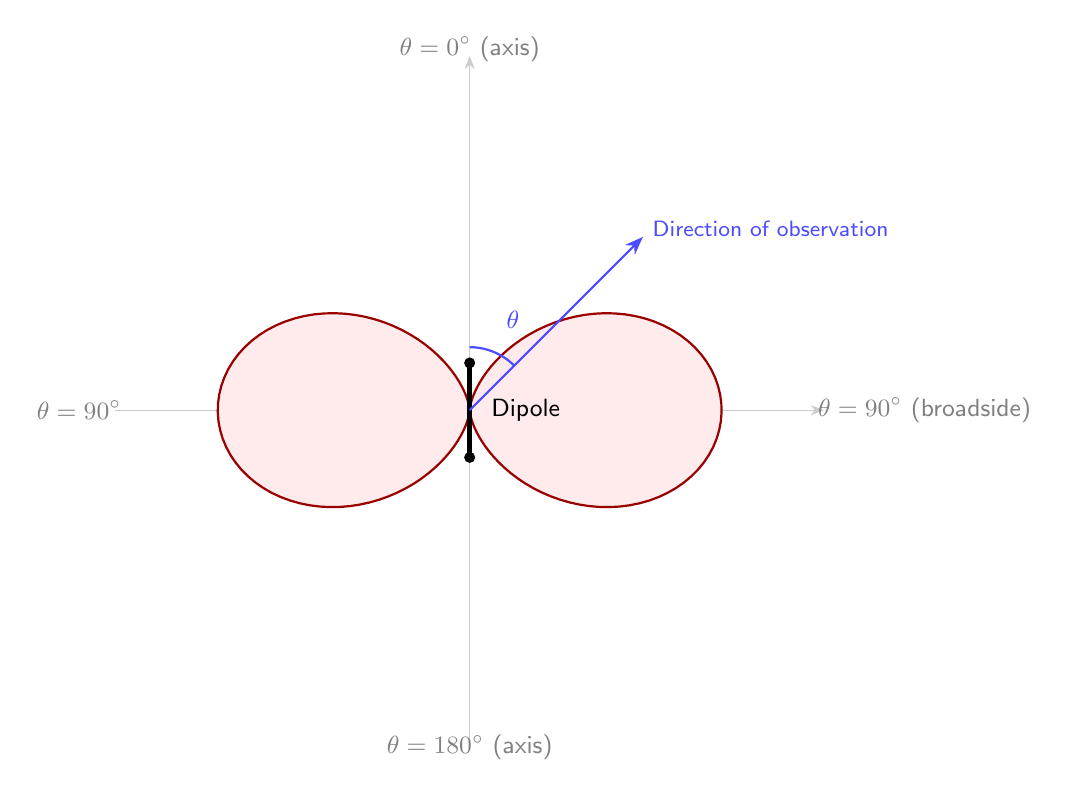
\begin{tikzpicture}[
    every node/.style={font=\sffamily\normalsize},
    >=Stealth
]

% --- Coordinate axes (faint) ---
\draw[thin, gray!40, ->] (0,-4.2) -- (0,4.5);
\draw[thin, gray!40, ->] (-4.5,0) -- (4.5,0);

% --- Radiation pattern (sin^2 theta in polar) ---
% In 2D cross-section: r(theta) = sin^2(theta)
% x = r*sin(theta), y = r*cos(theta) with scaling
\draw[thick, red!60!black, fill=red!8, domain=0:360, samples=180]
    plot ({3.2*sin(\x)*sin(\x)*sin(\x)}, {3.2*sin(\x)*sin(\x)*cos(\x)});

% --- Dipole antenna (center, vertical) ---
\draw[ultra thick, black] (0,-0.6) -- (0,0.6);
\fill[black] (0,-0.6) circle (2pt);
\fill[black] (0,0.6) circle (2pt);
\node[right, font=\sffamily\small] at (0.15,0) {Dipole};

% --- Theta angle definition ---
\draw[->, thick, blue!70] (0,0) -- (2.2, 2.2);
\draw[thick, blue!70] (0,0.8) arc (90:45:0.8);
\node[font=\sffamily\small, blue!70] at (0.55,1.15) {$\theta$};
\node[right, font=\sffamily\footnotesize, blue!70] at (2.2, 2.3) {Direction of observation};

% --- Axis labels ---
\node[above, font=\sffamily\small, gray] at (0,4.3) {$\theta = 0^\circ$ (axis)};
\node[below, font=\sffamily\small, gray] at (0,-4.0) {$\theta = 180^\circ$ (axis)};
\node[right, font=\sffamily\small, gray] at (4.3,0) {$\theta = 90^\circ$ (broadside)};
\node[left, font=\sffamily\small, gray] at (-4.3,0) {$\theta = 90^\circ$};

% --- Axis labels annotate structure without revealing answers ---
% Pattern shape (sin^2 theta) is visible — students interpret it themselves

\end{tikzpicture}
\end{document}
